%\chapter{Numerical Examples}
\chapter{実験・考察}

構成したSIBMを以下の実験環境(表\ref{table:sibm_env})で実装し、データの生成時間やデータベースシステムとのアクセス時間について考察を行う。

\begin{table}[h]
	\begin{center}
	\begin{tabular}{| l  p{45mm} |}
		\hline
		\rowstyle{\bfseries}
		実験環境 & \\
		\hline
		Operation System & Windows 8.1 Pro 64 bits \\
		CPU & Intel core i7 3770, 4 cores 8 thread @ 3.4Ghz (Boostable up to 3.9Ghz)
		\\
		RAM & 16GB \\
		Storage & HDD \\
		Java & 1.7.0\_71 (64 bits) \\
		Apache Jena & 2.12.1 \\
		SIBM & v0.9 build 20150129 \\
		\hline
	\end{tabular}
	\caption{実験環境}
	\label{table:sibm_env}
	\end{center}
\end{table}

SIBMを用いて生成したデータが図\ref{fig:sibm_sample}のような形になる。
	
\begin{figure}[h!]
	\lstinputlisting{./sample/sample.txt}
  	\caption{実装例}
  	\label{fig:sibm_sample}
\end{figure}

大数の避難場所情報を生成する場合、かかった時間やデータ量などの情報が表\ref{table:sibm_time_table}のようになる。

\begin{table}[h!]
	\begin{center}
	\begin{tabular}{| r | r | r | r | r | r |}
		\hline
		\rowstyle{\bfseries}
		避難場所数 & 生成時間(ms) & 関係者数 & トリプル数 & 挿入時間(ms) & サイズ(MB) \\
		\hline
		5 & 3373 & 1455 & 20409 & 3807 & 203.87 \\
		\hline
		10 & 4779 & 3018 & 42304 & 3669 & 205.57 \\
		\hline
		20 & 6783 & 6082 & 85482 & 5588 & 223.91 \\
		\hline
		50 & 7603 & 12645 & 177991 & 8312 & 296.59 \\
		\hline
		100 & 6591 & 24751 & 348443 & 12662 & 379.90 \\
		\hline
		200 & 10363 & 53719 & 755895 & 22522 & 625.34 \\
		\hline
		350 & 24708 & 112888 & 1584015 & 43468 & 1127.90 \\
		\hline
		500 & 30228 & 152903 & 2148284 & 55275 & 1456.53 \\
		\hline
		700 & 42229 & 220201 & 3091954 & 77798 & 2004.87 \\
		\hline
	\end{tabular}
	\caption{避難場所数に対する生成時間}
	\label{table:sibm_time_table}
	\end{center}
\end{table}

図\ref{fig:sibm_data_time}でわかるように、避難場所数が生成時間や人数・トリプル数と比例関係が確認できる。

\begin{figure}[t!]
 	\begin{center}
 		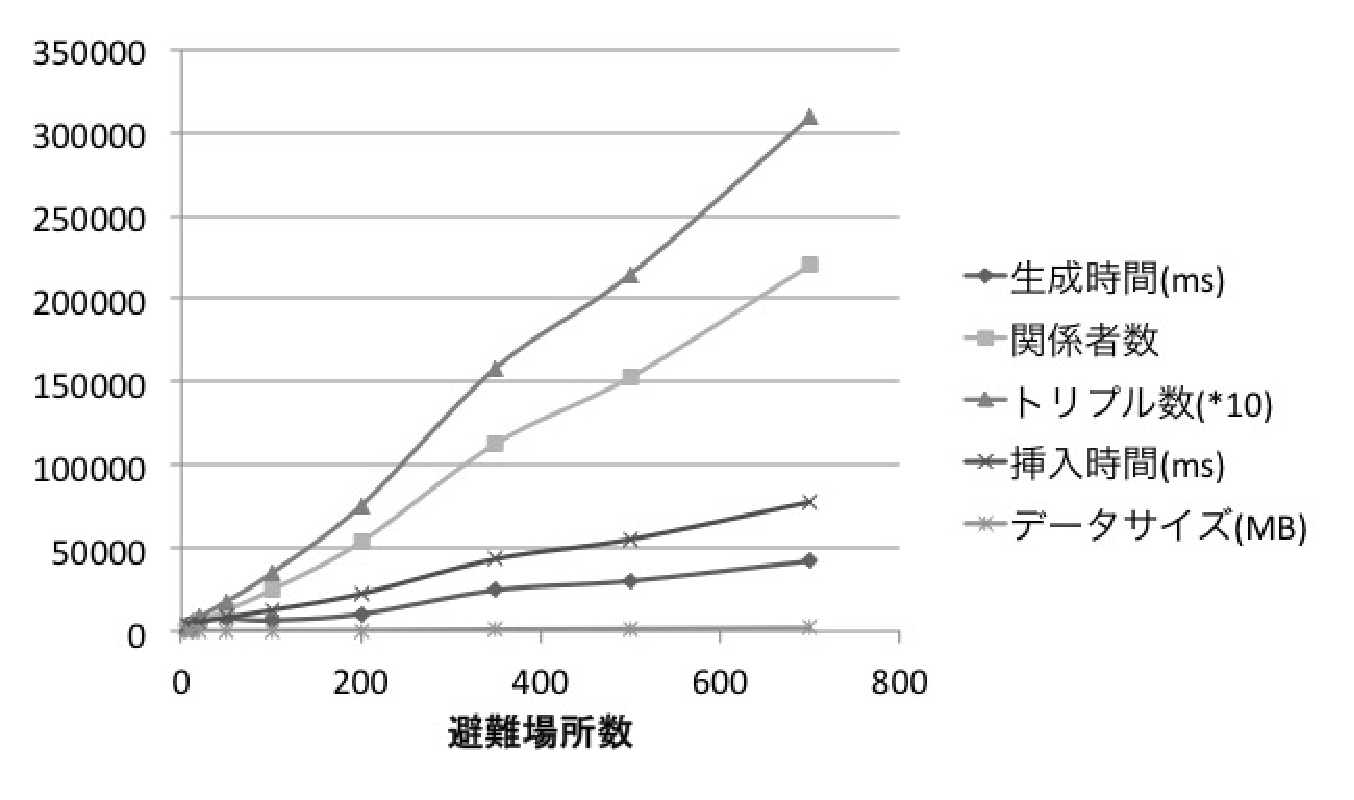
\includegraphics[width=120mm]{./images/test_chart1.eps}
 		\caption{生成・挿入時間とデータサイズ}
 		\label{fig:sibm_data_time}
 	\end{center}
\end{figure}

次に、生成したデータに対するクエリを行い、応答時間につい考察する。
なお、使用したクエリが\ref{appendix1}に説明する。また、Jena/TDBをデータストレージとして使用した。
実行時間をグラフ化した物は以下の図\ref{fig:sibm_query_time}のようになる。

\begin{figure}[t!]
 	\begin{center}
 		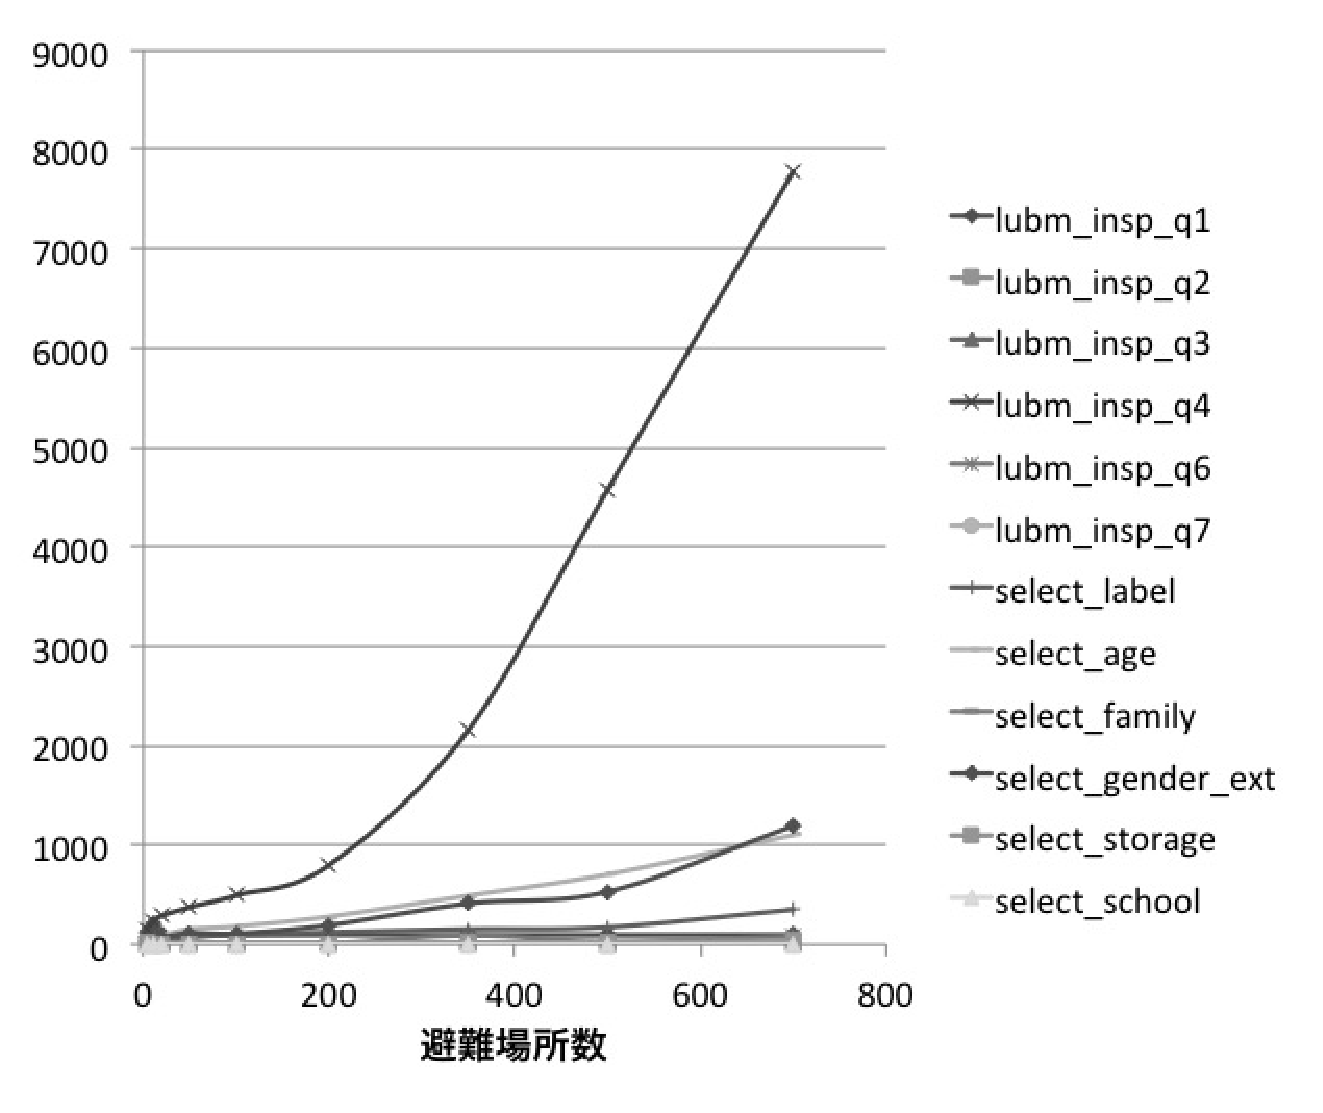
\includegraphics[width=120mm]{./images/test_query1.eps}
 		\caption{クエリ時間}
 		\label{fig:sibm_query_time}
 	\end{center}
\end{figure}

SIBMでは、特定なパラメーターに対する避難場所情報のRDFデータセットを生成することができ、現実に近い情報の元で実験を行うことが可能である。
このセッションでは、SIBMで生成したデータセットとそのもとのパラメーターとの反映性について考察する。また、生成した情報の実用性について考察する。

SIBMバージョン1で対応した入力値は避難場所の数である。SIBMが生成できる最大の数は12.5万となる。
ここでは、生成したデータをJena/TDBデータベースに挿入する時間と挿入後のデータサイズ・トリプル数について考察を行う。
入力した避難場所に対する挿入時間とデータ量が表\ref{table:sibm_time_table}になる。
避難場所の関係者数を避難場所の規模による計算される。その数によって人間情報を生成する。
表\ref{table:sibm_time_table}で示すように、避難場所の数に応じた関係者の数がわかる。

避難場所数とそれに対するデータ生成・挿入時間の関係が図\ref{fig:sibm_data_time}に示す。
生成されたデータ量(関係者数、トリプル数、データサイズ)が避難場所数に対して線形関係があることが考えられる。
だが、トリプル数/避難場所数の関係線が曲線になる。その理由は、特定な避難場所数に対して、生成しようとする関係者の数は定数ではなく、
ある範囲以内でランダムな数値で生成する。関係者情報に対するトリプル数と避難場所情報に対するトリプル数の総数では、ランダム性を持つため、
直線な関係にならないからである。

また、Jena/TDBデータベースでは、挿入するデータに対するメタデータやインデクシングすることによる発生したデータが多い。
そのため、少量データに対してもデータベースサイズが192.0MBになることがわかる\footnote{https://jena.apache.org/documentation/tdb/architecture.html}。

図\ref{fig:sibm_data_time}でわかるように、実際に発生する災害やそれに対する避難情報の増加が問題である。
例えば、北海道には約9000避難場所がある。実際に全てを使用する要求がでると、多量な情報が発生することが考えられる。そして、災害が短時間で発生することが多いため、
その短時間で多量なデータへの対策が事実な問題だとわかる。SIBMで生成するデータを使用し、その問題を解決する候補を実験することができる。
